\section{Local System}
\label{sec:test-ls}

The Local System is the most critical and more susceptible subsystem to cause errors. The probability of one error occur is bigger than on the other two subsystems and that's why this system is the one that needs to perform more test cases to be in the best performance possible.

The test cases can be divided in two main parts: hardware tests and software tests.

\subsection{Hardware Tests}
\label{subsec:ls-hw-tests}
%
There are many parts of hardware that need to be tested:
\begin{item-c}
\item Ultrasonic Sensors;
\item Fragrance Diffusion (Actuator and Module);
\item Camera;
\item Speakers;
\item Screen;
\end{item-c}

\subsubsection{Ultrasonic Sensors}
\label{sec:ussensors}

The ultrasonic sensors need to be with strong connections to all the supply sources and \gls{gpio} pins, after that, it has been ran a driver program that returned if the two sensors detected the presence of an obstacle. 
This program has a specific sample time that is more than enough to detect the presence of something in front of the sensors.
In fig.~\ref{fig:sensors-test} is the cable management of the sensors, while in fig.~\ref{fig:sensors-out-test} is the test output that ran as expected.
%
\begin{figure}[htb!]
  \centering
  \begin{subfigure}{.4\textwidth}
    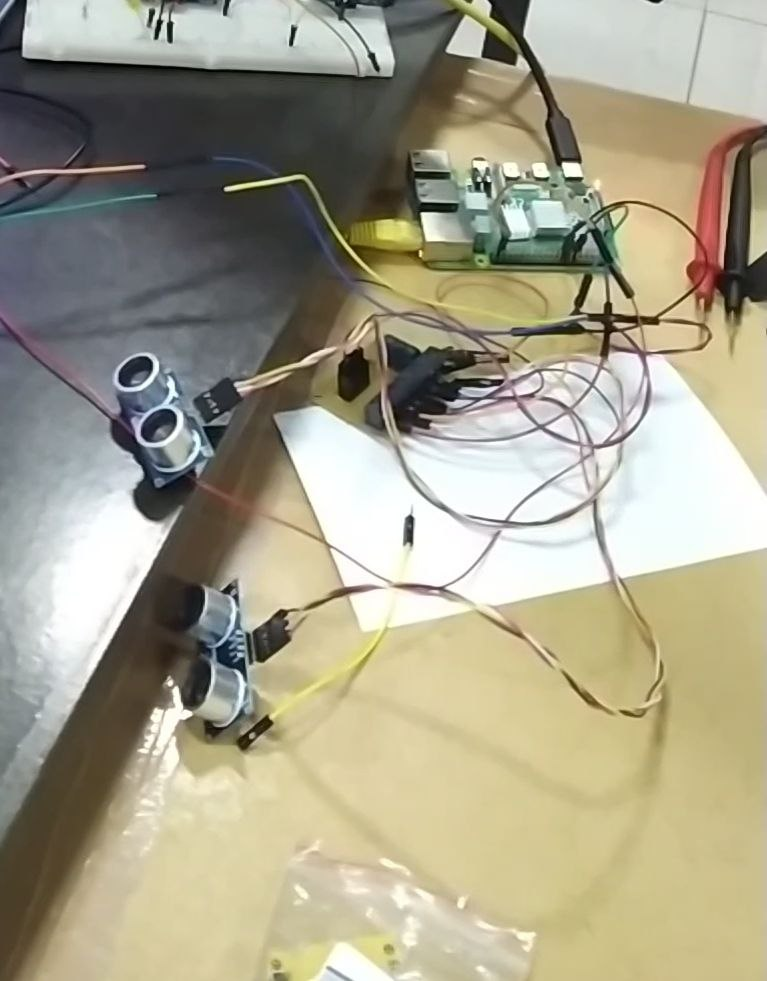
\includegraphics[width=\textwidth]{img/sensors-test.jpg}%
  \caption{Sensors Cable Management}%
  \label{fig:sensors-test}
  \end{subfigure}
  % 
  \begin{subfigure}{.5\textwidth}
    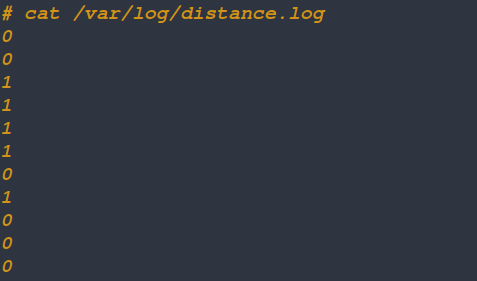
\includegraphics[width=\textwidth]{img/sensors-out-test.jpg}%
  \caption{Sensors Output Test}%
  \label{fig:sensors-out-test}
  \end{subfigure}
  % 
  \caption{Ultrasonic Sensors Test Cases}%
  \label{fig:uss-test}
\end{figure}

\subsubsection{Fragrance Diffusion (Actuator and Module)}
\label{sec:frag}

The fragrance diffuser module and its respective actuator need to be tested in order to respond to some signals gave by the main board.
In order for this to happen, it was tested with a driver program on the board and with all the module and it's components and the result was, as it can be seen in Fig.~\ref{fig:frag-test} what one expected.

\begin{figure}[!htb]
    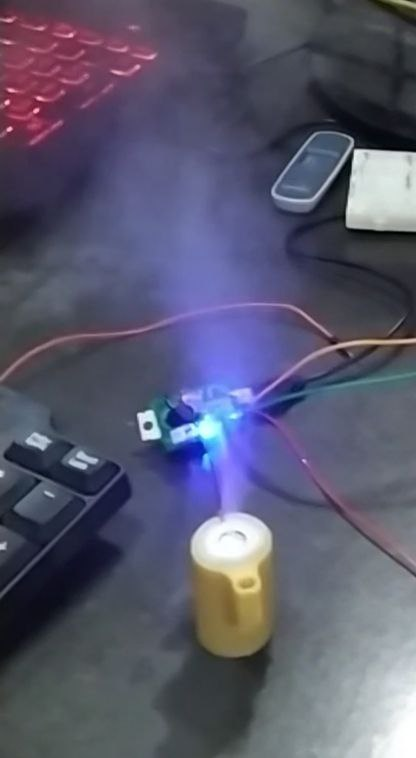
\includegraphics[width=.3\textwidth]{img/frag-test.jpg}%
  \caption{Fragrance Diffuser Output Test}%
  \label{fig:frag-test}
  \end{figure}
  
  
\subsubsection{Camera}
\label{sec:camera-test}
  
For the interaction mode it is mandatory that the camera module works properly to take pictures and gifs.
For this piece of hardware the test case is simple: turn on the camera and try to take a photo.

In this case it was used an image of Raspbian and with the help of an online app, the test of the camera worked as well as expected.
The result is on Fig.~\ref{fig:camera-test}.

\begin{figure}[!htb]
    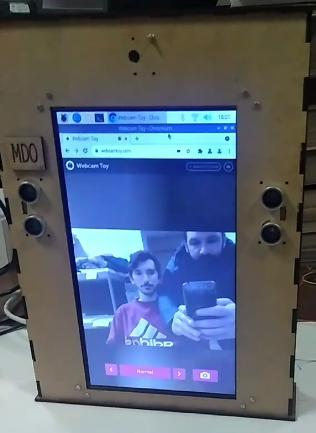
\includegraphics[width=.45\textwidth]{img/camera-teste.jpg}%
  \caption{Camera Output Test}%
  \label{fig:camera-test}
  \end{figure}
  
\subsubsection{Speakers}
\label{sec:speakers-test}

The speakers test cases are in a certain way different to test, because there's no way to show how it worked. However, the test was as simple as connect the speakers to the screen module board and play a video or an audio.

The audio played perfectly and the sound was well detected by human ears.

\subsubsection{Screen}
\label{sec:screen-test}

Testing the screen is similar to test the speakers. It's just simply connect the screen to the board and test its execution. As it can be seen in the previous figure when testing the camera (Fig.~\ref{sec:camera-test}) the screen was already being tested and it's more than proved that the screen works with no problems.


In conclusion, all hardware components and modules were tested successfully, which means that all test cases are now validated and it is possible to take the next step.
%%% Local Variables:
%%% mode: latex
%%% TeX-master: "../../../dissertation"
%%% End:
